\documentclass{article}
\usepackage{tikz}
\usepackage{CJKutf8}
\usepackage{amsmath}
\usepackage{amsthm}
\begin{document}
\begin{CJK}{UTF8}{gbsn}
\newtheorem*{Exercise}{习题}
  \begin{Exercise}
      画出具有$4$个顶点的所有无向图(同构的只算一个)。  
  \end{Exercise}
   { \centering
  \begin{minipage}{0.24\linewidth}
    \centering
    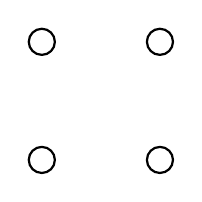
\begin{tikzpicture}[auto,
    specification/.style ={circle, draw, thick}]
   \node[specification] (A) at (0,0)  {};
   \node[specification] (B)  at (0,1.5)  {};
   \node[specification] (C)  at (1.5,1.5)  {};
   \node[specification] (D) at (1.5,0)  {};
 \end{tikzpicture}\\
 \vspace*{0.5cm}
 A
\end{minipage}\hfill
  \begin{minipage}{0.24\linewidth}
    \centering
    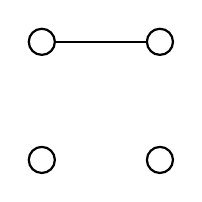
\begin{tikzpicture}[auto,
    specification/.style ={circle, draw, thick}]
   \node[specification] (A) at (0,0)  {};
   \node[specification] (B) at (0,1.5)  {};
   \node[specification] (C) at (1.5,1.5)  {};
   \node[specification] (D) at (1.5,0)  {};
   \draw[thick] (B) to  (C);
 \end{tikzpicture}\\
 \vspace*{0.5cm}
 B
\end{minipage}\hfill
  \begin{minipage}{0.24\linewidth}
    \centering
    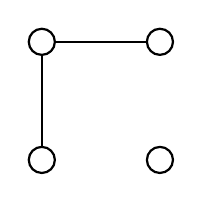
\begin{tikzpicture}[auto,
    specification/.style ={circle, draw, thick}]
   \node[specification] (A) at (0,0)  {};
   \node[specification] (B) at (0,1.5)  {};
   \node[specification] (C) at (1.5,1.5)  {};
   \node[specification] (D) at (1.5,0)  {};
   \draw[thick] (A) to  (B);
   \draw[thick] (B) to  (C);
 \end{tikzpicture}\\
 \vspace*{0.5cm}
 C
\end{minipage}\hfill
  \begin{minipage}{0.24\linewidth}
    \centering
    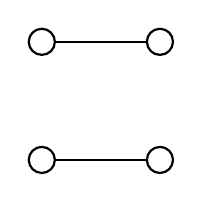
\begin{tikzpicture}[auto,
    specification/.style ={circle, draw, thick}]
   \node[specification] (A)  at (0,0)  {};
   \node[specification] (B)  at (0,1.5)  {};
   \node[specification] (C)  at (1.5,1.5)  {};
   \node[specification] (D) at (1.5,0)  {};
   \draw[thick] (B) to  (C);
   \draw[thick] (D) to  (A);
 \end{tikzpicture}\\
 \vspace*{0.5cm}
 D
\end{minipage}\hfill

\vspace*{0.5cm}
  \begin{minipage}{0.24\linewidth}
    \centering
    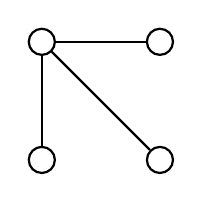
\begin{tikzpicture}[auto,
    specification/.style ={circle, draw, thick}]
   \node[specification] (A) at (0,0)  {};
   \node[specification] (B)  at (0,1.5)  {};
   \node[specification] (C)  at (1.5,1.5)  {};
   \node[specification] (D) at (1.5,0)  {};
   \draw[thick] (A) to (B);
   \draw[thick] (B) to (C);
      \draw[thick] (B) to (D);
 \end{tikzpicture}\\
 \vspace*{0.5cm}
 E
\end{minipage}\hfill
  \begin{minipage}{0.24\linewidth}
    \centering
    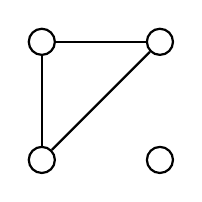
\begin{tikzpicture}[auto,
    specification/.style ={circle, draw, thick}]
   \node[specification] (A) at (0,0)  {};
   \node[specification] (B) at (0,1.5)  {};
   \node[specification] (C) at (1.5,1.5)  {};
   \node[specification] (D) at (1.5,0)  {};
   \draw[thick] (A) to  (B);
   \draw[thick] (B) to (C);
      \draw[thick] (C) to (A);
 \end{tikzpicture}\\
 \vspace*{0.5cm}
 F
\end{minipage}\hfill
  \begin{minipage}{0.24\linewidth}
    \centering
    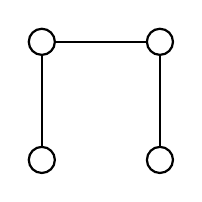
\begin{tikzpicture}[auto,
    specification/.style ={circle, draw, thick}]
   \node[specification] (A) at (0,0)  {};
   \node[specification] (B) at (0,1.5)  {};
   \node[specification] (C) at (1.5,1.5)  {};
   \node[specification] (D) at (1.5,0)  {};
   \draw[thick] (A) to  (B);
   \draw[thick] (B) to  (C);
      \draw[thick] (C) to (D);
 \end{tikzpicture}\\
 \vspace*{0.5cm}
 G
\end{minipage}\hfill
  \begin{minipage}{0.24\linewidth}
    \centering
    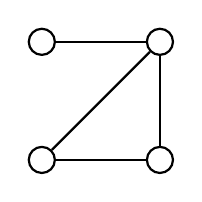
\begin{tikzpicture}[auto,
    specification/.style ={circle, draw, thick}]
   \node[specification] (A)  at (0,0)  {};
   \node[specification] (B)  at (0,1.5)  {};
   \node[specification] (C)  at (1.5,1.5)  {};
   \node[specification] (D) at (1.5,0)  {};
   \draw[thick] (A) to  (C);
   \draw[thick] (C) to  (D);
   \draw[thick] (D) to (A);
   \draw[thick] (C) to (B);
 \end{tikzpicture}\\
 \vspace*{0.5cm}
 H
\end{minipage}\hfill

\vspace*{0.5cm}
\flushleft
  \begin{minipage}{0.24\linewidth}
    \centering
    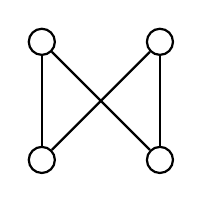
\begin{tikzpicture}[auto,
    specification/.style ={circle, draw, thick}]
   \node[specification] (A) at (0,0)  {};
   \node[specification] (B)  at (0,1.5)  {};
   \node[specification] (C)  at (1.5,1.5)  {};
   \node[specification] (D) at (1.5,0)  {};
   \draw[thick] (A) to (B);
   \draw[thick] (B) to (D);
   \draw[thick] (D) to (C);
      \draw[thick] (C) to (A);
 \end{tikzpicture}\\
 \vspace*{0.5cm}
 I
\end{minipage}
  \begin{minipage}{0.24\linewidth}
    \centering
    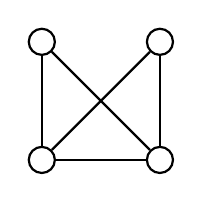
\begin{tikzpicture}[auto,
    specification/.style ={circle, draw, thick}]
   \node[specification] (A) at (0,0)  {};
   \node[specification] (B) at (0,1.5)  {};
   \node[specification] (C) at (1.5,1.5)  {};
   \node[specification] (D) at (1.5,0)  {};
   \draw[thick] (A) to  (B);
      \draw[thick] (C) to (D);
   \draw[thick] (D) to (A);
   \draw[thick] (A) to (C);
   \draw[thick] (B) to (D);
 \end{tikzpicture}\\
 \vspace*{0.5cm}
 J
\end{minipage}
  \begin{minipage}{0.24\linewidth}
    \centering
    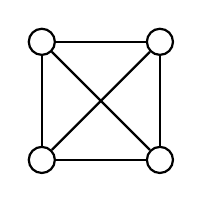
\begin{tikzpicture}[auto,
    specification/.style ={circle, draw, thick}]
   \node[specification] (A) at (0,0)  {};
   \node[specification] (B) at (0,1.5)  {};
   \node[specification] (C) at (1.5,1.5)  {};
   \node[specification] (D) at (1.5,0)  {};
   \draw[thick] (A) to  (B);
   \draw[thick] (B) to  (C);
      \draw[thick] (C) to (D);
   \draw[thick] (D) to (A);
   \draw[thick] (A) to (C);
   \draw[thick] (B) to (D);
 \end{tikzpicture}\\
 \vspace*{0.5cm}
 K
\end{minipage}
}

\begin{Exercise}
  画出具有$3$个顶点的所有有向图(同构的只算一个)。
\end{Exercise}
\begin{Exercise}
  画出具有$4$个、$6$个、$8$个顶点的三次图。
\end{Exercise}
\begin{Exercise}
  某次宴会上,许多人互相握手,证明:握过奇数次手的人数为偶数(注意,$0$为偶数)。
\end{Exercise}
\begin{Exercise}
  设$u$与$v$为图$G$的两个不同的顶点,若$u$与$v$间有两条不同的通道(迹),则$G$中是否有圈?
\end{Exercise}
  \begin{Exercise}
  若$G$是一个$(p,q)$图,$q > \frac{1}{2}(p-1)(p-2)$,试证$G$是连通图。  
  \end{Exercise}
  \begin{proof}[证明]
    用反证法。假设$G$不连通,则至少有两个连通分量。设其中一个连通分量的顶点数为
    $p_1$,边数为$q_1$,所有其他连通分量的顶点数为$p_2$,边数为$q_2$。则
    \begin{equation*}
      \begin{split}
        &\frac{1}{2}(p-1)(p-2)\\
        =&\frac{1}{2}(p_1 + p_2 -1)(p_1 + p_2 -2)\\
        =&\frac{1}{2}(p_1 + p_2 -1)((p_1 - 1) + (p_2 - 1))\\
        =&\frac{1}{2}(p_1(p_1 -1) +  p_1(p_2 - 1) + p_2(p_1 - 1) + p_2(p_2-1) - (p_1 - 1) - (p_2-1))\\
        =&\frac{1}{2}(p_1(p_1 -1) +   p_2(p_2-1) + 2(p_1 - 1)(p_2-1))\\
        =&\frac{p_1(p_1 -1)}{2} +   \frac{p_2(p_2-1)}{2} + (p_1 - 1)(p_2-1))\\
        \geq&\frac{p_1(p_1 -1)}{2} +   \frac{p_2(p_2-1)}{2}\\
        \geq & q
      \end{split}
    \end{equation*}
    矛盾。
  \end{proof}


  \begin{Exercise}
  证明:一个连通的$(p,q)$图中$q\geq p - 1$。  
  \end{Exercise}
  \begin{proof}[证明]
    设$G$为一个连通图,有$p$个顶点,$q$条边。如果$G$中有圈,去掉该圈上的一条边,得到的图仍然为连通的。如果所得到的图中还有圈,再去掉该圈上的一条边,得到的图还是连通的。如此进行下去,最后可以得到一个连通无圈的图。假设该连通无圈的图中有$q'$条边,如果能够证明$q'=p-1$,则结论得证。

    因此,只需证明一个连通无圈的$(p,q)$图中$q=p-1$即可。设$T$为一个连通无圈的$(p,q)$图,以下用数学归纳法证明$q=p-1$。

    
  (证法一)
  
    用数学归纳法证明,施归纳于顶点数$p$。
    
    (1)当$p=1$时,$q=0$,结论显然成立。

    (2)假设当$p=k$时结论成立,往证当$p=k+1$时结论也成立。设$T$有$k+1$个顶点。$T$中一定存在一个度为1的顶点,这是因为,设$P$为$T$中的一条最长
    路,$v$为$P$的一个端点,则$v$除了$P$上与其关联的边之外,由$T$中无圈知$v$不能再有其他的与$P$上的顶点相关联的边,同时由$P$为一条最长路知$v$不能再有与$P$外
    的顶点相关联的边,因此$v$的度必为1。去掉$T$中一个度为1的顶点及其与之关联的边,得到的图$T'$连通且无圈。$T'$有$k$个顶点,$q-1$条边,由归纳假设,$q-1 = k - 1$, 从而$q = (k +1) - 1$, 即当$p=k+1$时结论也成立。

    (证法二)
    
      用数学归纳法证明,施归纳于边数$q$。
    
    (1)当$q=0$时,$p=1$,结论显然成立。

    (2)假设当$q<k$时结论成立,往证当$q=k$时结论也成立。设$T$有$k$条边。去掉
    $T$中的任意一条边,得到两个支$T_1$和$T_2$,它们均连通无圈。设$T_1$有$p_1$个顶点,
    $k_1$条边,$T_2$有$p_2$个顶点,$k_2$条边,由归纳假设,
    \begin{equation*}
      \begin{split}
        k_1 &= p_1 - 1\\
        k_2 &= p_2 - 1
      \end{split}
    \end{equation*}
    以上两式相加,两边再同时加1,得
    \[k_1 + k_2  + 1 = p_1 + p_2 - 1\]
    从而
    \[k = p - 1 \]
    即当$q=k$时结论也成立。
\end{proof}

\begin{Exercise}
  在一个有$n$个人的宴会上,每个人至少有$m$个朋友($2\leq m < n$),试证:有不少于$m+1$个人,使得他们按照某种方法坐在一张圆桌旁,每人的左右均是他的朋友。
\end{Exercise}
  \begin{Exercise}
  设$G$为图。证明:若$\delta(G)\geq 2$,则$G$包含长度至少为$\delta(G)+1$的圈。  
  \end{Exercise}
  \begin{proof}[证明]
    设$P=v_0v_1\ldots v_n$为$G$中的一条最长路,则$v_0$只能与$P$中的顶点相邻接,否则假设$v_0$与不在$P$中的顶点$u$邻接,则$uv_0v_1\ldots v_n$构成了$G$中一条更长的路,与$P$为$G$中的最长路矛盾。取最大的$s$使得$v_0$与$v_s$相邻接,则$C=v_0v_1\ldots v_sv_0$为长度至少为$\delta(G)+1$的圈,这是因为$v_0$至少与$\delta(G)$个顶点相邻接,而所有这些与$v_0$邻接的顶点均在圈$C$中。
  \end{proof}

  \begin{Exercise}
    证明:如果$G$不是连通图,则$G^c$是连通图。
  \end{Exercise}

  \begin{Exercise}
    每一个自补图有$4n$或$4n+1$个顶点。
  \end{Exercise}
  \begin{Exercise}
    给出一个$10$个顶点的非哈密顿图的例子,使得每一对不邻接的顶点的$u$和$v$,均有:$\deg u + \deg v \geq 9$。
  \end{Exercise}
  \begin{Exercise}
    试求$K_p$中不同的哈密顿圈的个数。
  \end{Exercise}

  \begin{Exercise}
    完全偶图$K_{m,n}$为哈密顿图的充分必要条件是什么?
  \end{Exercise}

  \begin{Exercise}
    证明:具有奇数顶点的偶图不是哈密顿图。
  \end{Exercise}
  
\end{CJK}
\end{document}
%%% Local Variables:
%%% mode: latex
%%% TeX-master: t
%%% End:
